\chapter{Formatos}
%
\section{Fuente}
La fuente se elige mediante el archivo \textit{01-fuente-y-geometria.tex}, cargando el paquete específico de la fuente deseada; se configuran en las líneas mostradas en la figura \ref{fig:fuente}.
	\begin{figure}[H]
		\centering
		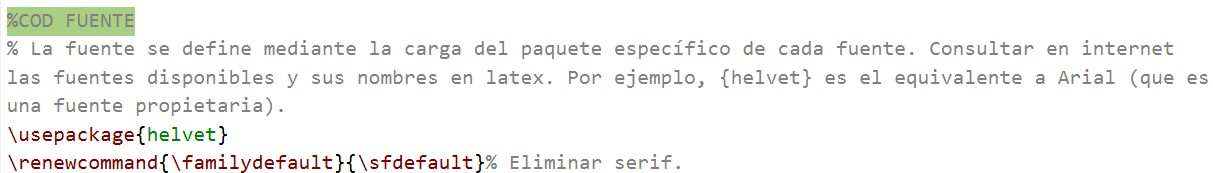
\includegraphics[width=1\linewidth, frame]{cuerpo/cap-redaccion/imagenes/fuente}
		\caption[Tipo de fuente.]{Tipo de fuente. Archivo: .../01-fuente-y-geometria.tex. Por defecto la plantilla usa \textit{helvetic} sin serif.}
		\label{fig:fuente}
	\end{figure}
%
\section{Tamaño de fuente y página}
Se configuran en el archivo raíz del \LaTeX{} (\textit{.../raiz.tex}), según la imagen \ref{fig:fuente-tamano}.
\begin{figure}[H]
	\centering
	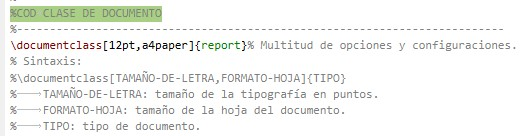
\includegraphics[width=1\linewidth, frame]{cuerpo/cap-redaccion/imagenes/fuente-tamano}
	\caption[Tamaño de letra y página.]{Tamaño de letra y página. Archivo: .../raíz.tex.}
	\label{fig:fuente-tamano}
\end{figure}
%
\subsection{Páginas a una o dos caras}
Se configura en el comando anterior (\ref{fig:fuente-tamano}).
%
\section{Márgenes, interlineado y otros espaciados.}
Se modifican mediante el archivo \textit{01-fuente-y-geometria.tex}, en las líneas mostradas en la figura \ref{fig:margenes-interlineado}.
\begin{figure}[H]
	\centering
	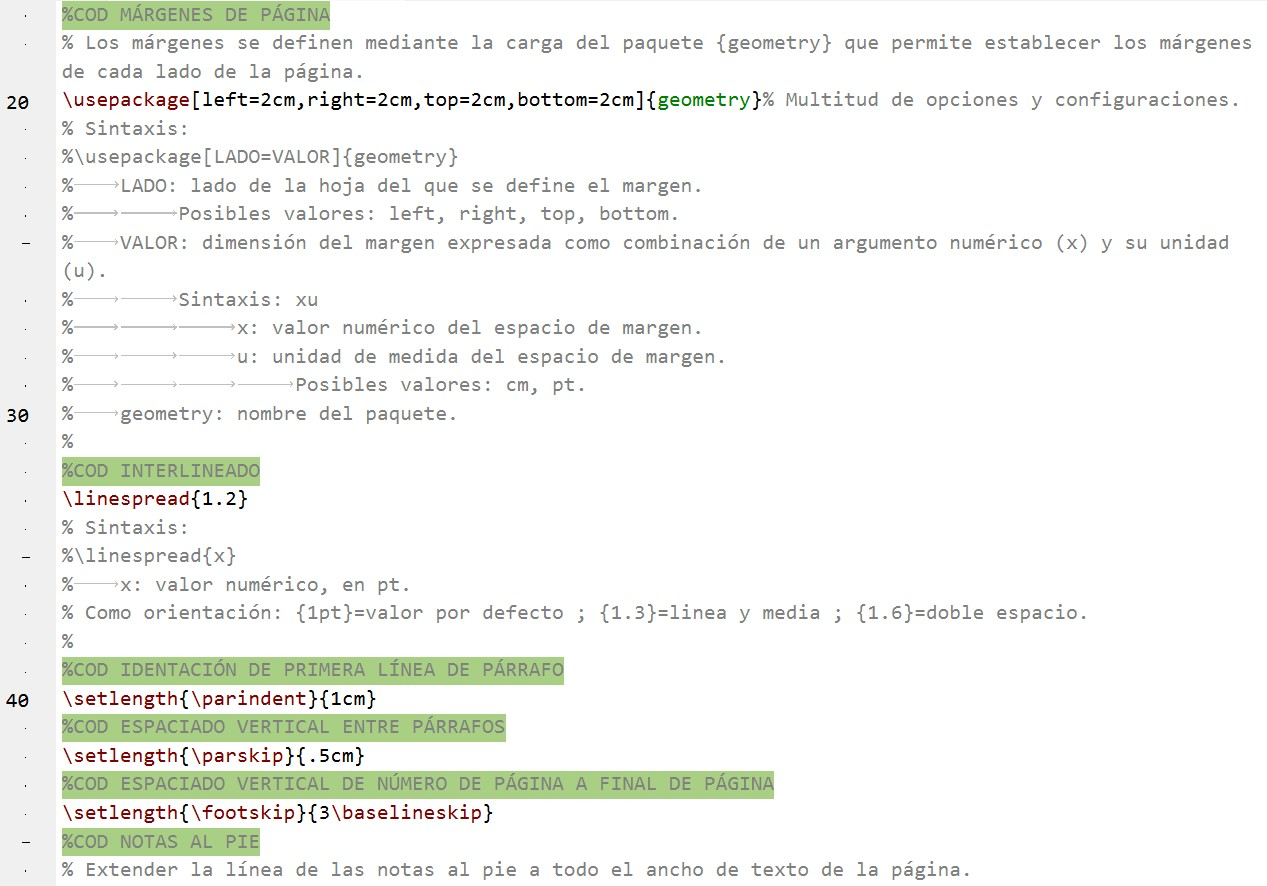
\includegraphics[width=1\linewidth, frame]{cuerpo/cap-redaccion/imagenes/margenes-interlineado}
	\caption[Márgenes e interlineado.]{Márgenes e interlineado. Archivo: .../01-fuente-y-geometria.tex.}
	\label{fig:margenes-interlineado}
\end{figure}
%
\section{Encabezados y pie de página}
Se emplea el paquete \href{https://www.ctan.org/pkg/fancyhdr}{\textit{fancyhdr}}. La configuración se implementa en el archivo .../03-encabezados.tex.
%
\section{Colores}
%
\subsection{Color de la fuente}
%
\subsubsection{Con \textit{\textbackslash color}}
Sintaxis: \textit{\textbackslash color\{COLOR\}}.

Establece el color para todo el texto a partir de ser declarado; para volver al color negro debe declararse explícitamente de nuevo con \textit{black} como argumento.
%
\subsubsection{Con \textit{\textbackslash textcolor}}
Sintaxis: \textit{\textbackslash textcolor\{COLOR\}\{TEXTO\}}.

Modifica solo el texto que se indica en el comando.
%
\subsection{Resalte de texto}
Sintaxis: \textbackslash \textit{hlc[COLOR]\{TEXTO\}}.

Modifica solo el texto que se indica en el comando.
%
\subsection{Ejemplos de cambios de color}
Esta linea debiera ser en color negro estándar.

\color{red}
Este linea debiera ser en color rojo.

Esta linea debiera ser en color negro estándar; pero es roja porque sigue activo el comando \textbackslash \textit{color\{red\}} que se declaró para la linea anterior.

\textcolor{green}{Esta linea debiera ser verde; porque se ha escrito dentro de un comando \textbackslash \textit{textcolor\{green\}}.}

Esta linea debiera ser en color negro estándar; pero es roja porque sigue activo el comando \textbackslash \textit{color\{red\}} que se declaró para la primera linea roja.

\color{brown}
Esta linea es marrón porque se ha declarado un \textbackslash \textit{color\{brown\}}.

\textcolor{purple}{Esta linea es púrpura; porque se ha escrito dentro de un comando \textbackslash \textit{textcolor\{purple\}}.}

\hlc[orange]{Esta linea tiene fuente marrón por el comando \textbackslash \textit{color\{brown\}} anterior; está resaltada en naranja por haber aplicado un comando \textbackslash \textit{hlc[orange]}}

\color{black}
Esta linea es negra porque se ha declarado un \textbackslash \textit{color\{black\}}.

\hlc[cyan]{Esta linea tiene fuente negra por haber restablecido el negro en la linea anterior; está resaltada en cian por haber aplicado un comando \textbackslash \textit{hlc[cyan]}.}

El código empleado es el mostrado en la figura \ref{fig:colores-codigo}.
\begin{figure}[h]
	\centering
	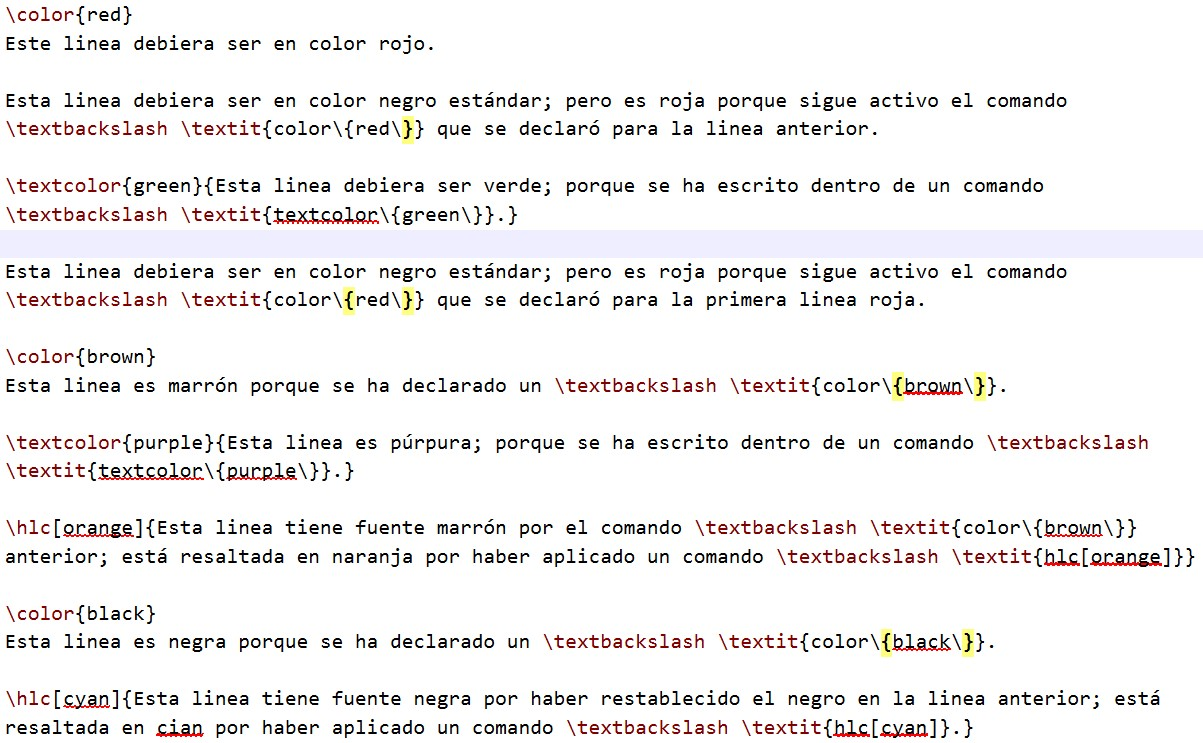
\includegraphics[width=1\linewidth, frame]{cuerpo/cap-redaccion/imagenes/colores-codigo}
	\caption[Colores y resalte de texto.]{Colores y resalte de texto.}
	\label{fig:colores-codigo}
\end{figure}
%
\subsection{Color de enlaces}
Es una configuración para todo el \LaTeX{} que se define en el archivo \textit{.../99-enlaces.tex}, como parte del paquete \href{https://www.ctan.org/pkg/hyperref}{\textit{hyperref}}, según se muestra en la imagen \ref{fig:color-enlaces}.
\begin{figure}[H]
	\centering
	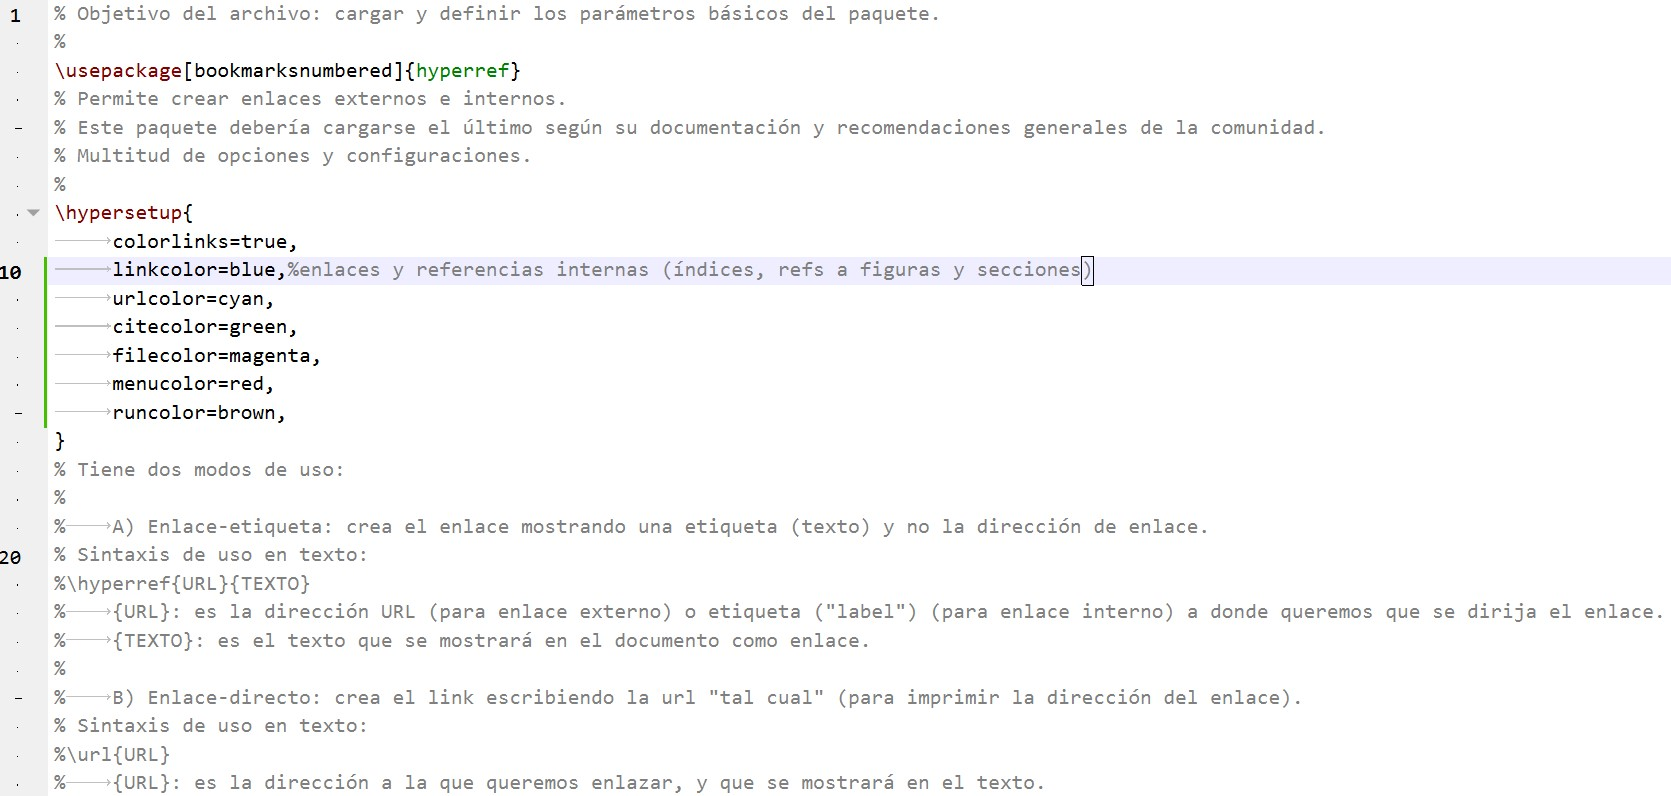
\includegraphics[width=1\linewidth, frame]{cuerpo/cap-redaccion/imagenes/color-enlaces}
	\caption[Color de enlaces.]{Color de enlaces. Archivo: .../99-enlaces.tex.}
	\label{fig:color-enlaces}
\end{figure}
%
\subsection{Color de la página}
Sintaxis: \textit{\textbackslash pagecolor\{COLOR\}}.

Establece el color a partir de ser insertado para el resto del documento, para volver al color blanco debe declararse explícitamente con \textbackslash\textit{nopagecolor}.